\section{WebGL}
\label{sec:chapter_tecnologie_abilitanti_webgl}
WebGL (Web Graphics Library) è una API Javascript che permette il rendering interattivo su browser web senza il bisogno di installare plug-in aggiuntivi.
Esso è integrato completamente come standard web in tutti i browser che permettono l’utilizzo dell’ accellerazione GPU per il rendering di immagini 2D e 3D.
Risulta compatibile con la maggior parte dei moderni browser disponibili sul mercato (figura: \ref{fig:stato_arte_webgl_compat}).
\\
\begin{figure}[htb]
 \centering
 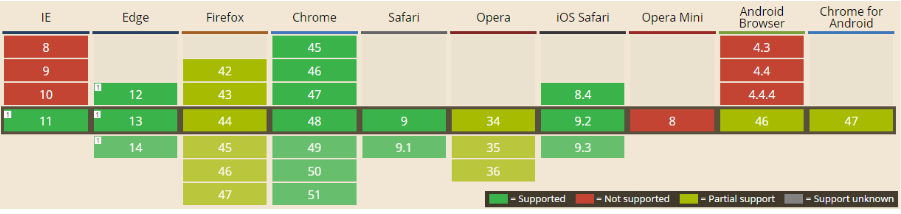
\includegraphics[width=1\linewidth]{images/chapter_tecnologie_abilitanti/tecnologie_abilitanti_webgl_compat.png}\hfill
 \caption[Lista browser compatibili]{Browser compatibili con WebGL.}
 \label{fig:stato_arte_webgl_compat}
\end{figure}
\\
WebGL si basa sulle \emph{OpengGL ES 2.0}, librerie grafiche OpenGL ottimizzate per dispositivi mobili, che forniscono un’ interfaccia di programmazione per la grafica 3D. Utilizza l’ elemento canvas HTML5, che viene acceduto attraverso il DOM (Document Object Model), per renderizzare l’ immagine desiderata.
\\
Le API WebGL sono di basso livello e funzionano intuitivamente come una sequenza di messaggi da inviare all’ oggetto gl che rappresenta un contesto WebGL costruito su una canvas.
\begin{lstlisting}[language=JavaScript]
gl=document.getElementById("canvas_id").getContext("experimental-webgl");
\end{lstlisting}
Analizzare la pipeline di rendering di WebGL equivale praticamente ad analizzare la pipeline di OpenGL ES 2.0. Grazie a WebGL il programmatore non deve preoccuparsi dell’ intero processo di rendering in quanto alcune delle fasi più complesse vengono gestite dalla libreria.
La pipeline di WebGL è implementata per mezzo di Shader programmabili seguendo le specifiche di OpenGL ES 2.0 e di GLSL. Quest’ultimo è un linguaggio di programmazione ad alto livello per la gestione delle unità di shader di una GPU.
\\
Per shader si intende un’ insieme di istruzioni software che permettono di definire particolari operazioni ed effetti, come colorazione ed illuminazione, per il rendering degli elementi 3D della scena.
\\
In figura \ref{fig:tecnologie_abilitanti_webglrender}  è possibile osservare la pipeline di WebGL.La pipeline risulta simile a quella analizzata precedentemente in capitolo \ref{sec:chapter_stato_arte_open_gl}, ma presenta alcune differenze negli Shader.
\\
\begin{figure}[htb]
 \centering
 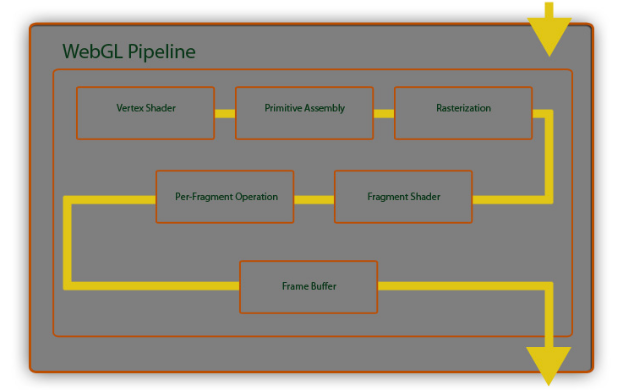
\includegraphics[width=0.9\linewidth]{images/chapter_tecnologie_abilitanti/tecnologie_abilitanti_webglrender.png}\hfill
 \caption[La pipeline di WebGL]{La pipeline di rendering WebGL}
 \label{fig:tecnologie_abilitanti_webglrender}
\end{figure}
\\
Le specifiche WebGL richiedono che lo sviluppatore provveda a fornire alla GPU due shader chiamati rispettivamente Vertex Shader e Fragment Shader:
\begin{itemize}
\item Il Vertex Shader è un metodo programmabile il cui compito è quello di restituire, per ogni tripletta di coordinate che identificano un vertice nello spazio, una coppia di coordinate che identifichino lo stesso vertice sul piano bidimensionale dello schermo (la canvas). Tale operazione prende in considerazione le informazioni come il punto di vista e l’angolazione dalla quale viene osservata la scena.
\item Il Fragment Shader è un metodo programmabile il cui compito è quello di definire il colore di ognuno dei pixel della canvas sulla quale giace la rappresentazione bidimensionale della scena calcolata con le informazione del Vertex Shader. Tramite esso è possibile implementare effetti d’ illuminazione, effettuare il texture mapping, applicare le ombre oppure effetti come la rifrazione, riflessione o il bump mapping.
\end{itemize}
WebGL utilizza un dialetto del linguaggio di programmazione C chiamato GLSL per la definizione degli shaders. Questo linguaggio è stato appositamente realizzato per svolgere questo compito e per essere facilmente integrato in una pagina web.
\\
Un esempio di fragment shader è il seguente:


\begin{lstlisting}[language=html]
<script id="shader--fs" type="x-shader/x-fragment">
\end{lstlisting}
\begin{lstlisting}[language=javascript]
void main(void){
	gl_FragColor = vec4(1.0,1.0,1.0,1.0);
}
\end{lstlisting}
\begin{lstlisting}[language=html]
</script>
\end{lstlisting}

GLSL richiede che nella variabile \texttt{gl\_FragColor} venga inserito il colore con il quale viene renderizzato a video il pixel in oggetto. Se si utilizzasse lo shader creato nell’esempio tot su un modello tridimensionale, esso verrebbe visualizzato di colore bianco.
\\
Un vertex shader segue lo stesso approccio; la variabile da valorizzare in questo caso è chiamata \texttt{gl\_Position}.

\begin{lstlisting}[language=javascript]
void main(void){
	gl_Position = uPMatrix * uMVMatrix * vec4(aVertexPositionm 1.0);
}
\end{lstlisting}

Il problema di WebGL risiede però nella sua complessità.
Per disegnare un semplice triangolo bianco è necessario dichiarare le coordinate dei punti (x,y,z) che compongono i vertici (nove valori nell’ esempio).
Questi valori devono poi essere memorizzati all’ interno di un buffer utilizzato durante la fase di disegno.

\begin{lstlisting}[language=javascript]
function initBuffers() {
	triangleVertexPositionBuffer = gl.createBuffer();
	gl.bindBuffer(gl.ARRAY_BUFFER, triangleVertexPositionBuffer);

	var vertices = [ 0.0, 1.0, ...];

	gl.bufferData(gl.ARRAY_BUFFER, new Float32Array(vertices), gl.STATIC_DRAW);
	triangleVertexPositionBuffer.itemSize = 3;
	triangleVertexPositionBuffer.numItems = 3;
}
\end{lstlisting}
Successivamente per effettuare il rendering della scena su schermo sono necessarie ulteriori operazioni:

\begin{lstlisting}[language=javascript]
function drawScene() {
	gl.viewport(0, 0, gl.viewportWidth, gl.viewportHeight);
	gl.clear(gl.COLOR_BUFFER_BIT | gl.DEPTH_BUFFER_BIT);
	gl.bindBuffer(gl.ARRAY_BUFFER, triangleVertexPositionBuffer);

	gl.vertexAttribPointer(
		shaderProgram.vertexPositionAttribute,
		triangleVertexPositionBuffer.itemSize,
		gl.FLOAT, false, 0, 0);

	gl.uniformMatrix4fv(shaderProgram.pMatrixUniform, false, new Float32Array([1,0,0,0,....]));

	gl.uniformMatrix4fv(shaderProgram.uMVMatrixUniform, false, new Float32Array([1,0,0,0,..]));

	gl.drawArrays(gl.TRIANGLES, 0, triangleVertexPositionBuffer.numItems);
}
\end{lstlisting}
La funzione \texttt{DrawScene} nell’ esempio gestisce le operazioni necessarie per disegnare il triangolo nella canvas; nelle prime due righe viene resettata la scena, poi viene caricato nel contesto 3D il buffer contenente le informazioni dei vertici del triangolo e vengono impostati i parametri richiesti dagli shader.
Infine viene invocata la funzione \texttt{drawArrays} che disegna i vertici presenti nel buffer invocando per ognuno di essi gli shader.
\\
L’ esempio fornito, volutamente non completo, non vuole essere una spiegazione esaustiva di come usare WebGl, piuttosto risulta utile al fine di comprenderne la complessità di utilizzo.
\\
Disegnare un solo triangolo bianco e statico (senza alcuna animazione) è costato infatti circa 60 righe; a queste bisogna aggiungere ulteriori istruzioni di gestione del contesto WebGl sulla canvas scelta.
Le API WebGL risultano quindi decisamente troppo complesse e laboriose da utilizzare, soprattutto per la realizzazione di scene complesse. Scene complesse, come gli appartamenti 3D arredati costruiti nel presente lavoro di tesi.
\\
Three.js nasce con l’obiettivo di risolvere i problemi appena esposti e per facilitare il lavoro dello sviluppatore.

